\chapter{El bloque p II: el oxígeno, los halógenos y los gases nobles}\label{ch:b1:p-block-16-18}

El ácido sulfúrico se fabrica en mayor tonelaje que cualquier otro
producto químico: disuelve la roca fosfática para los fertilizantes,
lixivia los minerales de cobre y de uranio, refina el petróleo y llena
las baterías de los coches, y durante un siglo la producción de ácido
sulfúrico fue una medida aproximada de la industria de un país. La mayor
parte de su azufre procede hoy de la depuración del gas natural y del
petróleo; una parte todavía se saca a mano de cráteres volcánicos. El
azufre está en el \omterm{def:b1:periodicity:table}{grupo} 16, debajo del oxígeno; los \omterm{def:b1:p-block-16-18:halogen}{halógenos} del \omterm{def:b1:periodicity:table}{grupo}
17 y los gases nobles del \omterm{def:b1:periodicity:table}{grupo} 18 completan el \omterm{def:b1:periodicity:table}{bloque} p. Este capítulo
sigue el oxígeno y el azufre desde el elemento hasta el ácido, ordena los
\omterm{def:b1:p-block-16-18:halogen}{halógenos} como \omterm{def:b1:nernst:couple}{oxidantes} con sus \omterm{def:b1:nernst:electrode-potential}{potenciales estándar}, y termina con los
compuestos que sí forman los gases nobles, supuestamente inertes.

\begin{recall}
Las \omterm{def:b1:lewis-resonance-vsepr:lewis}{estructuras de Lewis}, los octetos expandidos y las formas RPECV
(\cref{ch:b1:lewis-resonance-vsepr}); los \omterm{def:b1:nernst:electrode-potential}{potenciales estándar}
(\cref{ch:b1:nernst}); la \omterm{def:b1:e-ph-diagrams:disproportionation}{dismutación} del cloro y el \omterm{def:b1:e-ph-diagrams:e-ph-diagram}{diagrama
potencial--pH} del cloro (\cref{ch:b1:e-ph-diagrams}); la catálisis
(\cref{ch:b1:elementary-steps}). El volumen escolar (año 10) agrupó los
\omterm{def:b1:p-block-16-18:halogen}{halógenos} y los gases nobles en familias.
\end{recall}

\begin{omfigure}
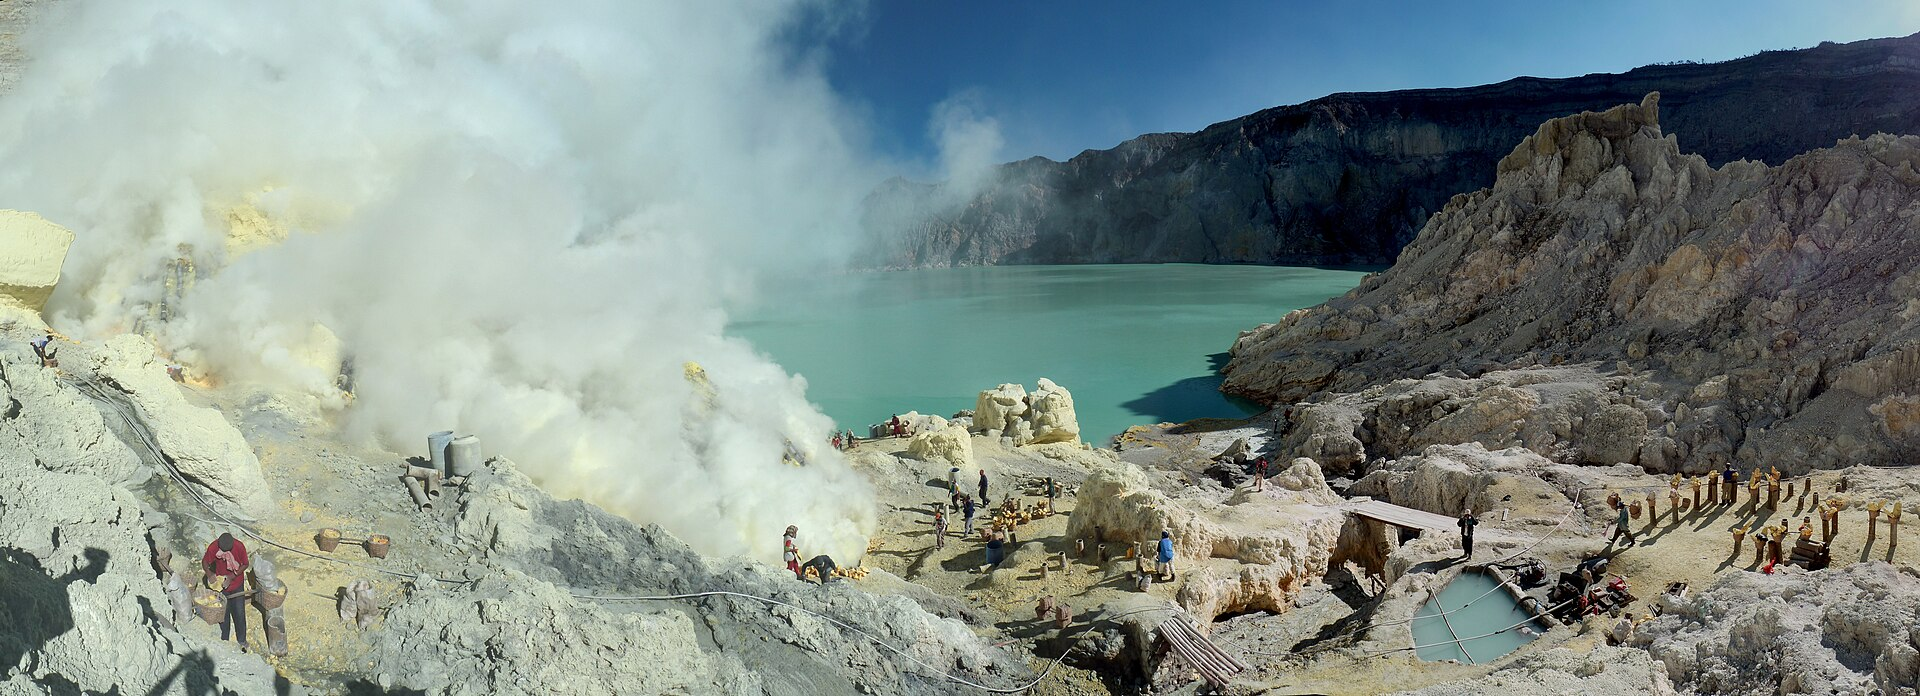
\includegraphics[width=0.78\linewidth]{images/book2/kawah-ijen.jpg}

{\small Extracción de azufre en el cráter del volcán Kawah Ijen
(Indonesia): los gases volcánicos condensan azufre amarillo alrededor de
unas tuberías, y los mineros lo sacan en cestos (fotografía de Sémhur,
CC BY-SA 4.0, Wikimedia Commons).}
\end{omfigure}

\section{El oxígeno, el ozono y los peróxidos}

\begin{definition}[Calcógenos]\label{def:b1:p-block-16-18:chalcogen}
Los \emph{calcógenos}\index{calcogeno@calcógeno} son los elementos del \omterm{def:b1:periodicity:table}{grupo} 16
(O, S, Se, Te, Po), con seis \omterm{def:b1:quantum-numbers:configuration}{electrones de valencia}
\textit{ns}$^2$\textit{np}$^4$. Forman compuestos con \omterm{def:b1:nernst:oxidation-number}{números de
oxidación} de $-$II (óxidos, sulfuros) a $+$VI (sulfatos), los más altos
solo a partir del azufre.
\end{definition}

El oxígeno existe como dioxígeno \ce{O2} y como ozono \ce{O3}, una
molécula angular con dos \omterm{def:b1:lewis-resonance-vsepr:resonance}{formas resonantes}
(\cref{ch:b1:lewis-resonance-vsepr}). El ozono es un \omterm{def:b1:nernst:couple}{oxidante} más fuerte
que el dioxígeno: $E^\circ(\ce{O3}/\ce{O2}) = 2.07$~V, frente a 1.23~V
para \ce{O2}/\ce{H2O}. En la alta atmósfera absorbe la luz ultravioleta;
cerca del suelo es un contaminante. El peróxido de hidrógeno, con un
enlace \ce{O-O} y el oxígeno en $-$I, es a la vez \omterm{def:b1:nernst:couple}{oxidante} y \omterm{def:b1:nernst:couple}{reductor}, y
se dismuta lentamente (\cref{exo:b1:nernst:12}).
% ledger: dfg:O3_g (E0 computed in figdata/bachelor-1/standard-potentials.py)

\begin{example}[Los números de oxidación del oxígeno]
El oxígeno, superado en \omterm{def:b1:periodicity:electronegativity}{electronegatividad} solo por el flúor, está en
$-$II en casi todos sus compuestos: el agua, los óxidos, los hidróxidos,
los sulfatos. Las excepciones se deducen de la regla según la cual los
electrones compartidos van al compañero más electronegativo y se reparten
a partes iguales entre átomos idénticos. En el peróxido de hidrógeno
\ce{H2O2}, H--O--O--H, cada oxígeno toma los electrones de su enlace
\ce{O-H}, pero comparte el par \ce{O-O}: $-$I. En el superóxido de potasio
\ce{KO2}, el ion \ce{O2-} lleva una carga para dos átomos: $-\frac12$ de
media. En el difluoruro de oxígeno \ce{OF2}, el flúor se queda con los
dos enlaces, y el oxígeno está en $+$II. En \ce{O2} y \ce{O3} está en 0.
Solo el estado $-$II es estable frente al agua; los peróxidos y los
superóxidos son \omterm{def:b1:nernst:couple}{oxidantes}, y el \ce{OF2}, un agente fluorante.
\end{example}

\section{El azufre y el ácido sulfúrico}

El azufre, a diferencia del oxígeno, forma anillos y cadenas de enlaces
sencillos \ce{S-S}: el azufre ordinario está formado por anillos \ce{S8}.
Arde dando dióxido de azufre, una molécula angular (ángulo O--S--O de
\ang{119.5}), que puede oxidarse más hasta trióxido de azufre, trigonal
plano. Ambos son \omterm{def:b1:s-block:oxide-character}{óxidos ácidos}: el \ce{SO2} da ácido sulfuroso
($\mathrm{p}K_a$ 1.77 y 7.22), y el \ce{SO3}, ácido sulfúrico.
% ledger: geo:SO2.aOSO, dfg:SO2_g, dfg:SO3_g

\begin{proposition}[Etapas del proceso de contacto]\label{prop:b1:p-block-16-18:contact-steps}
El ácido sulfúrico se fabrica a partir del azufre en cuatro etapas:
(1) \ce{S + O2 -> SO2}; (2) \ce{2SO2 + O2 <=> 2SO3}, sobre un
\omterm{def:b1:elementary-steps:catalyst}{catalizador} de óxido de vanadio(V); (3) \ce{SO3 + H2SO4 -> H2S2O7}
(óleum), absorbiéndose el trióxido en ácido concentrado;
(4) \ce{H2S2O7 + H2O -> 2H2SO4}. En conjunto,
\ce{2S + 3O2 + 2H2O -> 2H2SO4}.
\end{proposition}

\begin{proof}
Cada etapa está ajustada; al sumar $2\times(1)$, (2), $2\times(3)$ y
$2\times(4)$, se cancelan \ce{SO2}, \ce{SO3} y \ce{H2S2O7}, y los dos
\ce{H2SO4} consumidos en la etapa 3 se regeneran en la etapa 4, lo que
deja \ce{2S + 3O2 + 2H2O -> 2H2SO4}. La etapa 2 es termodinámicamente
muy favorable a temperatura ambiente ($K = 10^{24.8}$ a
\qty{25}{\celsius}, a partir de las energías de Gibbs de formación), pero
extremadamente lenta: es el \omterm{def:b1:elementary-steps:catalyst}{catalizador}, activo solo en caliente, el que
la hace avanzar, y el compromiso entre velocidad y conversión se estudia
en el volumen del segundo año. El \ce{SO3} no se absorbe directamente en
agua porque su reacción con el vapor de agua forma una fina niebla de
gotitas de ácido que atraviesa los absorbedores.
\end{proof}
% ledger: dfg:SO2_g, dfg:SO3_g

\begin{omfigure}
\begin{tikzpicture}[font=\small, >={Stealth}, box/.style={draw, rounded corners, fill=omDef!8, align=center, minimum height=1.0cm}]
  \node[box] (b) at (0,0) {quemador\\de azufre\\\ce{S + O2 -> SO2}};
  \node[box] (c) at (4.4,0) {convertidor, \ce{V2O5}\\lechos catalíticos};
  \node[box] (a) at (8.8,0) {torre de absorción\\\ce{SO3} en \ce{H2SO4}};
  \node[box] (d) at (8.8,-2.2) {dilución\\\ce{H2S2O7 + H2O}};
  \draw[<-, thick] (b.west) -- ++(-0.8,0) node[left] {aire, S};
  \draw[->, thick] (b) -- node[above] {\ce{SO2}} (c);
  \draw[->, thick] (c) -- node[above] {\ce{SO3}} (a);
  \draw[->, thick] (a) -- node[right] {óleum} (d);
  \draw[->, thick] (d.west) -- ++(-1.2,0) node[left] {\ce{H2SO4}};
  \draw[->, thick] (d.east) -- ++(0.6,0) |- node[pos=0.25, right] {retorno} (a.east);
\end{tikzpicture}

{\small El proceso de contacto: combustión del azufre, oxidación
catalítica del \ce{SO2}, absorción del \ce{SO3} en ácido sulfúrico
concentrado y dilución del óleum. Una parte del ácido vuelve al
absorbedor.}
\end{omfigure}

\begin{proposition}[Fuerza del ácido sulfúrico]\label{prop:b1:p-block-16-18:sulfuric-strength}
En agua, la primera acidez del ácido sulfúrico es fuerte (total), y la
segunda, débil: $\mathrm{p}K_a(\ce{HSO4-}/\ce{SO4^2-}) = 1.99$. Una
disolución de \qty{0.010}{mol/L} no está, por tanto, a pH 1.70 (dos
protones) ni a 2.00 (uno), sino en medio.
\end{proposition}

\begin{proof}
El \ce{H2SO4}, con dos oxígenos sin hidrógeno sobre el azufre, es un
\omterm{def:b1:p-block-13-15:oxoacid}{oxoácido} más fuerte que \ce{H3O+}: está nivelado
(\cref{ch:b1:predominant-reaction}). El \ce{HSO4-}, ya negativo, retiene
más su protón: su $\mathrm{p}K_a$, calculado a partir de las energías de
Gibbs de formación, es 1.99. Para $C = 0.010$: $[\ce{H3O+}] = C + x$,
$[\ce{HSO4-}] = C - x$, $[\ce{SO4^2-}] = x$, con
$x(C + x)/(C - x) = 10^{-1.99}$; resolviendo, $x = \qty{4.2e-3}{mol/L}$ y
$\mathrm{pH} = -\log(0.0142) = 1.85$.
\end{proof}
% ledger: dfg:HSO4-_ao, dfg:SO42-_ao

El ácido sulfúrico concentrado es también un potente agente deshidratante
(carboniza el azúcar, quitándole los elementos del agua) y, en caliente,
un \omterm{def:b1:nernst:couple}{oxidante}. Su dilución libera mucho calor: el ácido se vierte siempre
sobre el agua, nunca al revés. La mayor parte del azufre del mundo, unos
84 millones de toneladas en 2025, se recupera del sulfuro de hidrógeno
del gas natural y de las corrientes de refinería, y la mayor parte acaba
como ácido sulfúrico.
% ledger: usgs:S-world-2025

\begin{method}[Balance de materia a través del proceso de contacto]\label{met:b1:p-block-16-18:contact-balance}
\begin{enumerate}
  \item Se usa la ecuación global: un \ce{H2SO4} por cada átomo de S.
  \item Se corrige con la conversión de la etapa 2 (la fracción de
        \ce{SO2} oxidada) y con las pérdidas en la absorción.
  \item Para el aire: se calcula el \ce{O2} necesario (tres medios por
        cada S) y se divide por su fracción en el aire.
\end{enumerate}
\end{method}

\begin{example}[Una planta que quema mil toneladas de azufre al día]
Una planta quema \qty{1000}{t} de azufre al día, convierte el
\qty{99.0}{\percent} del \ce{SO2} y absorbe el \qty{99.9}{\percent} del
\ce{SO3}. Entonces $n(\ce{S}) = \num{1000e6}/32.1 = \qty{3.12e7}{mol}$ y
$n(\ce{H2SO4}) = \num{3.12e7} \times 0.990 \times 0.999
= \qty{3.08e7}{mol}$, es decir, $\num{3.08e7} \times \qty{98.1}{g}
= \qty{3020}{t}$ de ácido al día. El \qty{1.0}{\percent} no convertido
sale como \ce{SO2}: \qty{3.1e5}{mol}, o \qty{20}{t} al día, que hay que
eliminar del gas de cola. El dioxígeno necesario es
$1.5 \times \num{3.12e7} =
\qty{4.67e7}{mol}$; el aire, con un
\qty{21}{\percent} de \ce{O2}, son \qty{2.23e8}{mol}, o
$V = nRT/p = \qty{5.5e6}{m^3}$ al día a \qty{25}{\celsius} y
\qty{1}{bar}, antes del exceso que la planta insufla en realidad.
\end{example}
% ledger: air:O2

\section{Los halógenos}

\begin{definition}[Halógenos]\label{def:b1:p-block-16-18:halogen}
Los \emph{halógenos}\index{halogeno@halógeno} son los elementos del \omterm{def:b1:periodicity:table}{grupo} 17 (F, Cl,
Br, I, At), con siete \omterm{def:b1:quantum-numbers:configuration}{electrones de valencia}
\textit{ns}$^2$\textit{np}$^5$. Existen como moléculas diatómicas \ce{X2}
y forman iones haluro \ce{X-}.
\end{definition}

\begin{omfigure}
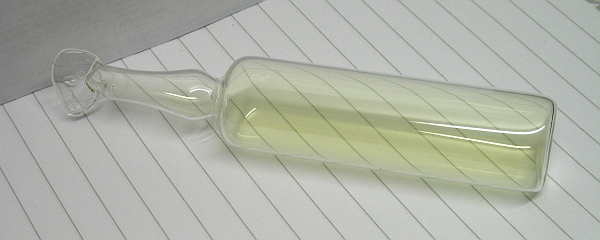
\includegraphics[height=2.9cm]{images/book2/chlorine.jpg}\hspace{0.5em}%
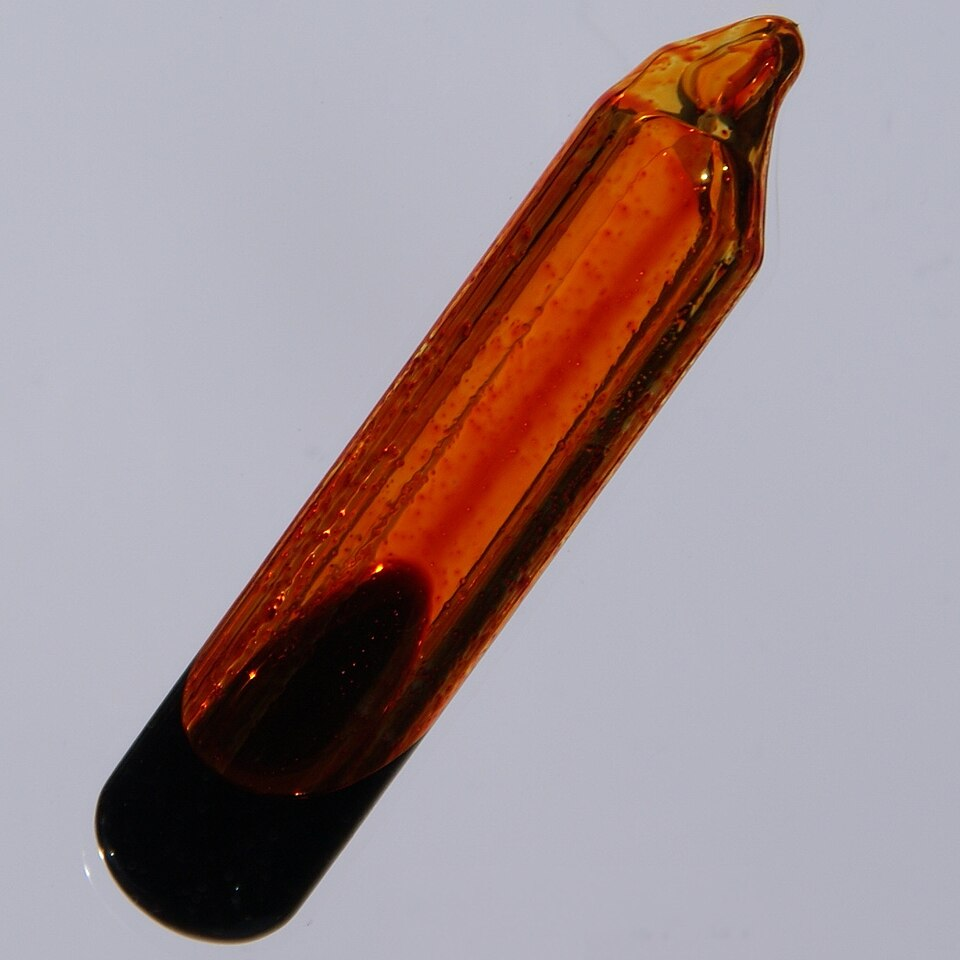
\includegraphics[height=2.9cm]{images/book2/bromine.jpg}\hspace{0.5em}%
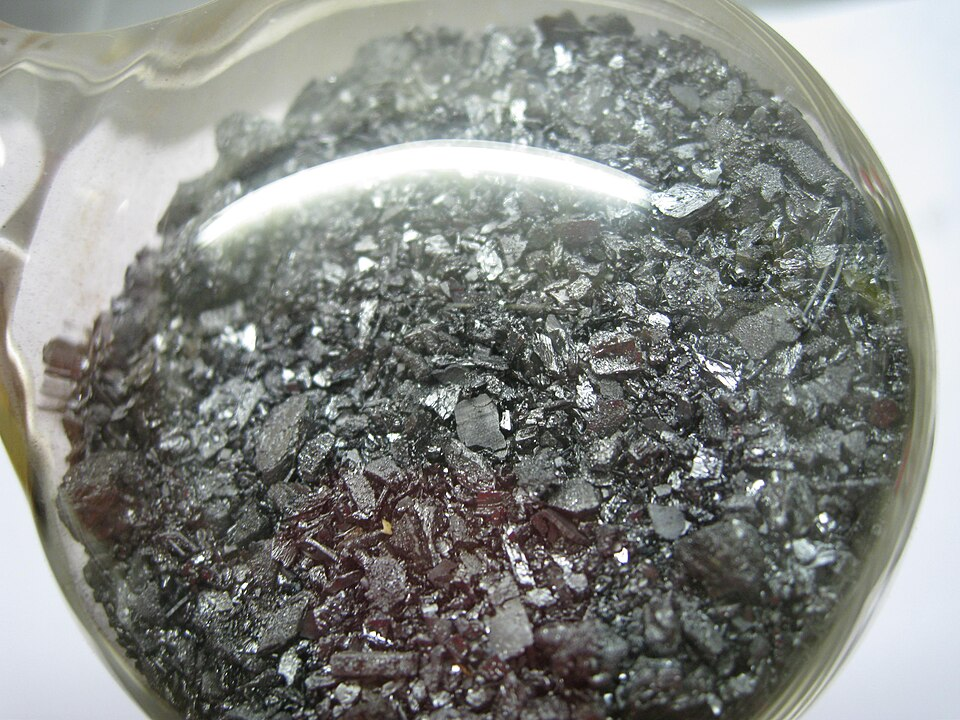
\includegraphics[height=2.9cm]{images/book2/iodine.jpg}

{\small El cloro, un gas amarillo verdoso pálido (W. Oelen, CC BY-SA
3.0); el bromo, un líquido rojo oscuro con un vapor naranja (Jurii, CC BY
3.0); el yodo, \omterm{def:b1:crystals-metals:crystal}{cristales} negro grisáceos de brillo metálico (Dnn87, CC BY
3.0). El cloro y el bromo están sellados en ampollas de vidrio. Todas de
Wikimedia Commons.}
\end{omfigure}

\begin{proposition}[Poder oxidante de los halógenos]\label{prop:b1:p-block-16-18:halogen-oxidising-order}
Los \omterm{def:b1:p-block-16-18:halogen}{halógenos} son \omterm{def:b1:nernst:couple}{oxidantes} cuya fuerza disminuye al descender por el
grupo:
$E^\circ(\ce{F2}/\ce{F-}) = 2.89$~V, \ce{Cl2}/\ce{Cl-} 1.36~V,
\ce{Br2}/\ce{Br-} 1.08~V, \ce{I2}/\ce{I-} 0.53~V. Cada \omterm{def:b1:p-block-16-18:halogen}{halógeno} oxida los
iones haluro que están debajo de él en el grupo.
\end{proposition}

\begin{proof}
Los valores proceden de las energías de Gibbs de formación de los iones
haluro (\cref{ch:b1:nernst}). Según la regla de la gamma, \ce{X2} oxida
a \ce{Y-} cuando el par \ce{X2}/\ce{X-} está por encima de
\ce{Y2}/\ce{Y-}: por ejemplo,
\ce{Cl2 + 2Br- -> 2Cl- + Br2}, $\log K = 2(1.36 - 1.08)/0.059 = 9.5$.
Al descender por el grupo, los átomos crecen, disminuyen su afinidad por
un electrón adicional y la hidratación de los iones haluro, más pequeños
arriba, y con ellas el potencial.
\end{proof}
% ledger: dfg:F-_ao, dfg:Cl-_ao, dfg:Br-_ao, dfg:I-_ao

\begin{omfigure}
\begin{tikzpicture}
\begin{axis}[
  ybar, width=0.62\linewidth, height=5.0cm, ymin=0, ymax=3.3,
  symbolic x coords={F,Cl,Br,I}, xtick=data,
  xticklabels={\ce{F2}/\ce{F-}, \ce{Cl2}/\ce{Cl-}, \ce{Br2}/\ce{Br-}, \ce{I2}/\ce{I-}},
  ylabel={$E^\circ$ (V)}, bar width=16pt, nodes near coords,
  every node near coord/.append style={font=\scriptsize},
  tick label style={font=\small}, label style={font=\small}, enlarge x limits=0.2]
\addplot[fill=omThm!40, draw=omThm] coordinates {(F,2.89) (Cl,1.36) (Br,1.08) (I,0.53)};
\end{axis}
\end{tikzpicture}

{\small \omterm{def:b1:nernst:electrode-potential}{Potenciales estándar} de los pares halógeno--haluro a
\qty{25}{\celsius}, calculados a partir de energías de Gibbs tabuladas:
el poder \omterm{def:b1:nernst:couple}{oxidante} disminuye de forma regular al descender por el grupo.}
\end{omfigure}

Los haluros de hidrógeno son todos ácidos en agua, pero el \ce{HF} es
débil ($\mathrm{p}K_a$ 3.16), mientras que \ce{HCl}, \ce{HBr} y \ce{HI}
son fuertes: el enlace \ce{H-F} es muy fuerte, y el pequeño ion fluoruro
queda retenido por \omterm{def:b1:intermolecular-forces-solvents:hbond}{enlaces de hidrógeno} fuertes. El flúor es el elemento
más electronegativo y el \omterm{def:b1:nernst:couple}{oxidante} más fuerte de la tabla; solo se obtiene
por electrólisis. Los \omterm{def:b1:p-block-13-15:oxoacid}{oxoácidos} del cloro --- hipocloroso \ce{HClO},
clórico \ce{HClO3}, perclórico \ce{HClO4} --- son más fuertes cuantos más
oxígenos sin hidrógeno tienen, como todos los \omterm{def:b1:p-block-13-15:oxoacid}{oxoácidos}
(\cref{def:b1:p-block-13-15:oxoacid}); su relación con el cloruro y el
cloro se cartografió en el
\cref{ch:b1:e-ph-diagrams}.
% ledger: dfg:HF_ao, dfg:F-_ao

\begin{omfigure}
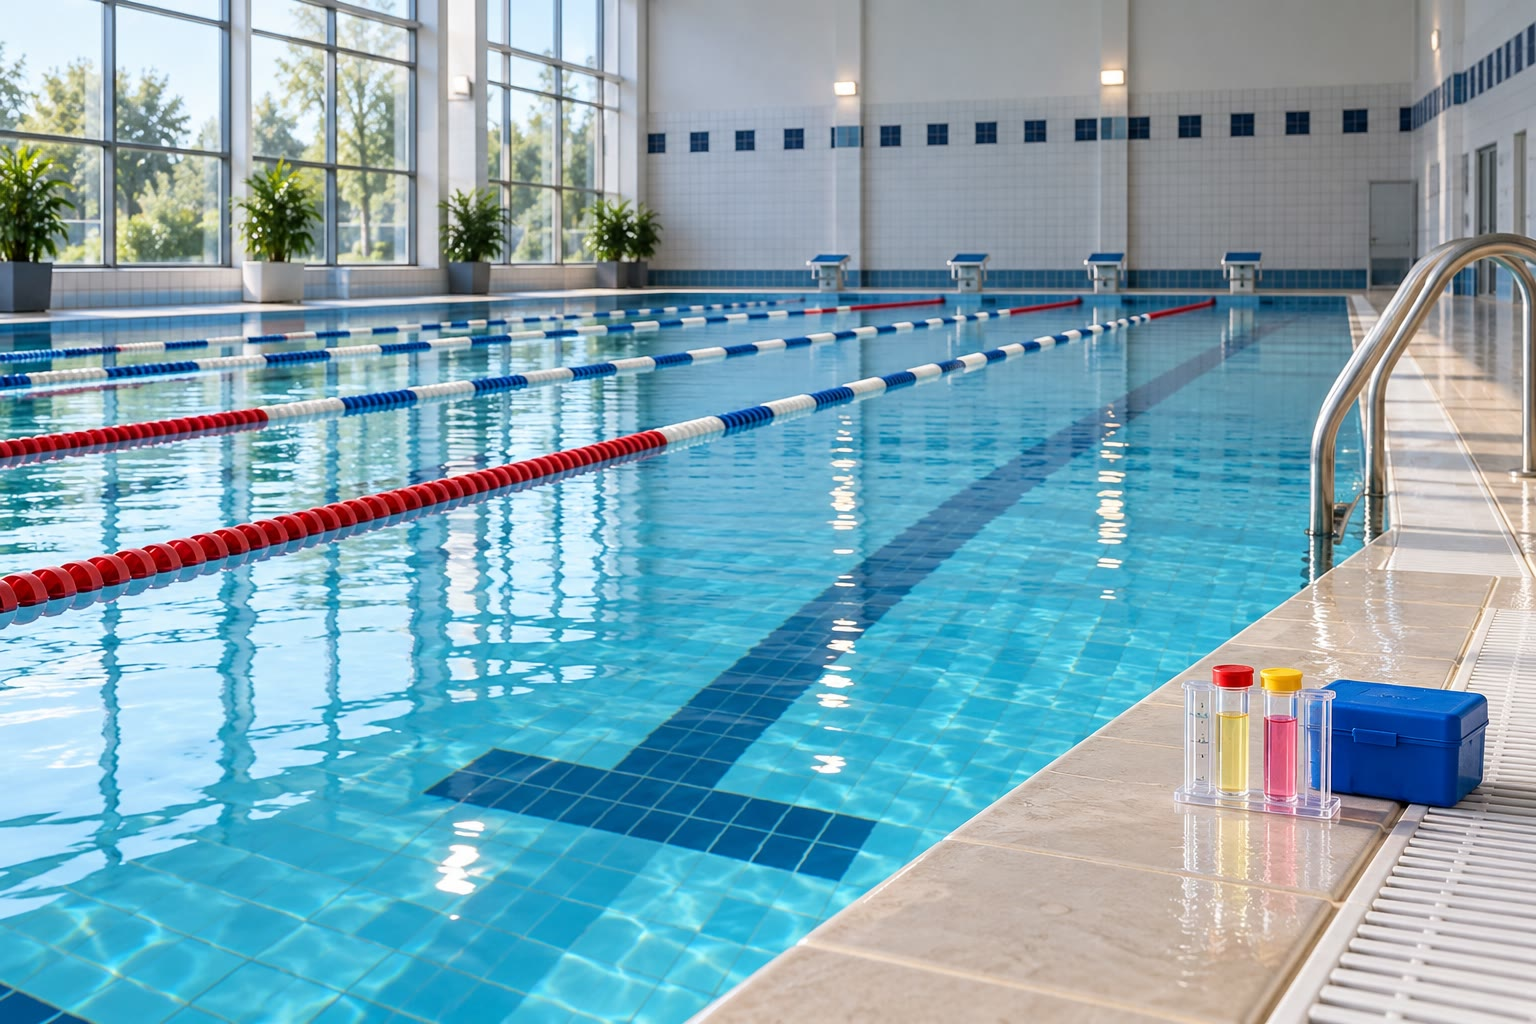
\includegraphics[width=0.55\linewidth]{images/book2/ai/b1-28-swimming-pool.jpg}

{\small Una piscina pública y su estuche de análisis del agua: el cloro
disuelto en forma de ácido hipocloroso se controla varias veces al día.}
\end{omfigure}

\begin{definition}[Compuestos interhalogenados]\label{def:b1:p-block-16-18:interhalogen}
Un \emph{compuesto interhalogenado}\index{compuesto interhalogenado} es un
compuesto de dos \omterm{def:b1:p-block-16-18:halogen}{halógenos} distintos: \ce{ICl}, \ce{BrF3}, \ce{ClF3},
\ce{IF7}. El \omterm{def:b1:p-block-16-18:halogen}{halógeno} más grande y menos electronegativo es el \omterm{def:b1:complexation:complex}{átomo
central}, con un octeto expandido a partir de \ce{ClF3}.
\end{definition}

\begin{inthelab}[Manipular los halógenos]
El cloro es tóxico y solo se prepara en pequeñas cantidades en una
vitrina de gases; el bromo quema la piel y su vapor ataca los pulmones,
y se usa diluido, en vitrina, con guantes y gafas, con una disolución de
tiosulfato de sodio a mano para destruir los derrames
(\ce{4Br2 + S2O3^2- + 5H2O -> 8Br- + 2SO4^2- + 10H+}). El yodo es el más
suave de los tres, pero mancha y sublima; se guarda en un frasco cerrado.
\end{inthelab}

\section{Los gases nobles y sus compuestos}

Los gases nobles (He, Ne, Ar, Kr, Xe, Rn) tienen las capas de valencia
llenas y las energías de ionización más altas de sus \omterm{def:b1:periodicity:table}{periodos}
(\cref{ch:b1:periodicity}). Considerados inertes durante mucho tiempo, los
más pesados, cuyos electrones externos están menos retenidos, sí
reaccionan con los elementos más electronegativos: el xenón da
\ce{XeF2}, \ce{XeF4}, \ce{XeF6} y óxidos. Sus formas siguen las reglas
RPECV, con \omterm{def:b1:lewis-resonance-vsepr:lewis}{pares no enlazantes} en el xenón.

\begin{example}[Por qué el xenón, y no el argón]
Las \omterm{def:b1:periodicity:ionisation-energy}{primeras energías de ionización} de los gases nobles disminuyen al
descender por el grupo: He 24.59, Ne 21.56, Ar 15.76, Kr 14.00, Xe 12.13,
Rn 10.75~eV. La del dioxígeno, \ce{O2 -> O2+ + e-}, es de 12.07~eV, casi
la misma que la del xenón. Un \omterm{def:b1:nernst:couple}{oxidante} lo bastante fuerte para arrancar
un electrón al \ce{O2}, dando el catión dioxigenilo \ce{O2+}, debería por
tanto oxidar también el xenón, pero no el argón, que retiene su electrón
3.7~eV más fuertemente. El xenón reacciona, en efecto, con el \omterm{def:b1:nernst:couple}{oxidante}
muy fuerte hexafluoruro de platino \ce{PtF6}, dando un sólido de
composición global \ce{XePtF6}, y con el propio flúor, que da los
fluoruros de xenón de la tabla siguiente. El radón, todavía más fácil de
ionizar, es demasiado radiactivo para que pueda hacerse mucha química con
él.
\end{example}
% ledger: ie:He, ie:Ne, ie:Ar, ie:Kr, ie:Xe, ie:Rn, ie:O2, lit:XePtF6

\begin{omfigure}
\begin{tabular}{llll}
\hline
molécula & pares del \omterm{def:b1:complexation:complex}{átomo central} & forma & ángulo medido \\
\hline
\ce{SO2} & 2 dominios enlazantes + 1 \omterm{def:b1:lewis-resonance-vsepr:lewis}{par no enlazante} & angular & \ang{119.5} \\
\ce{SF6} & 6 enlazantes & octaédrica & \ang{90} \\
\ce{ClF3} & 3 enlazantes + 2 no enlazantes & en forma de T & \ang{87.5} \\
\ce{XeF2} & 2 enlazantes + 3 no enlazantes & lineal & \ang{180} \\
\ce{XeF4} & 4 enlazantes + 2 no enlazantes & plano-cuadrada & \ang{90} \\
\hline
\end{tabular}

\smallskip
{\small Formas de algunas moléculas del \omterm{def:b1:periodicity:table}{bloque} p con octetos expandidos o
\omterm{def:b1:lewis-resonance-vsepr:lewis}{pares no enlazantes} (ángulos medidos, cuando se dispone de ellos). Los
\omterm{def:b1:lewis-resonance-vsepr:lewis}{pares no enlazantes} del \ce{XeF2} ocupan las tres posiciones ecuatoriales
de una bipirámide trigonal, lo que deja la molécula lineal.}
% ledger: geo:SO2.aOSO, geo:SF6.aFSF, geo:ClF3.aFClF, geo:XeF2.aFXeF
\end{omfigure}

El argón, casi un uno por ciento del aire, protege materiales reactivos en los
laboratorios y en la soldadura; el helio, procedente del gas natural,
enfría imanes superconductores, como los de los espectrómetros de RMN
(\cref{ch:b1:structure-spectroscopy}).
% ledger: air:Ar

\section{Ejercicios}

\begin{exercise}[$\star$]\label{exo:b1:p-block-16-18:1}
Dese el \omterm{def:b1:nernst:oxidation-number}{número de oxidación} del azufre en \ce{H2S}, \ce{S8}, \ce{SO2},
\ce{SO3^2-}, \ce{SO4^2-}, \ce{S2O3^2-} (medio) y \ce{H2S2O7}.
\end{exercise}

\begin{exercise}[$\star$]\label{exo:b1:p-block-16-18:2}
¿Cuáles de estas reacciones tienen lugar: el cloro con el yoduro de
potasio; el yodo con el bromuro de sodio; el bromo con el cloruro de
sodio; el cloro con el bromuro de sodio? Escríbanse las que tienen lugar.
\end{exercise}

\begin{exercise}[$\star$]\label{exo:b1:p-block-16-18:3}
Dibújense las \omterm{def:b1:lewis-resonance-vsepr:lewis}{estructuras de Lewis} de \ce{SO2}, \ce{SO3} y \ce{O3}, con
sus \omterm{def:b1:lewis-resonance-vsepr:resonance}{formas resonantes}, y dense sus formas.
\end{exercise}

\begin{exercise}[$\star$]\label{exo:b1:p-block-16-18:4}
Escríbanse las reacciones del \ce{SO2} y del \ce{SO3} con el agua y con
el hidróxido de sodio.
\end{exercise}

\begin{exercise}[$\star\star$]\label{exo:b1:p-block-16-18:5}
Calcúlese el pH del ácido fluorhídrico de \qty{0.10}{mol/L} y compárese
con el del ácido clorhídrico de la misma concentración. Explíquese la
diferencia.
\end{exercise}

\begin{exercise}[$\star\star$]\label{exo:b1:p-block-16-18:6}
Predíganse con el \omterm{def:b1:lewis-resonance-vsepr:vsepr}{modelo RPECV} las formas de \ce{BrF5}, \ce{IF7} (siete
\omterm{def:b1:lewis-resonance-vsepr:lewis}{pares enlazantes}, bipirámide pentagonal), \ce{ICl4-} y \ce{XeO3}.
\end{exercise}

\begin{exercise}[$\star\star$]\label{exo:b1:p-block-16-18:7}
Calcúlese la constante de \ce{Cl2 + 2I- -> 2Cl- + I2} y dígase por qué el
agua de cloro vuelve azul un papel de almidón--yoduro.
\end{exercise}

\begin{exercise}[$\star\star$]\label{exo:b1:p-block-16-18:8}
Demuéstrese que el ozono puede oxidar los iones yoduro a yodo y
escríbase la reacción en medio ácido. ¿Por qué se usa para medir el
ozono?
\end{exercise}

\begin{exercise}[$\star\star$]\label{exo:b1:p-block-16-18:9}
El ácido sulfúrico concentrado carboniza la sacarosa, \ce{C12H22O11}.
Escríbase la \omterm{def:b1:alcohol-activation:dehydration}{deshidratación} a carbono y calcúlese la masa de carbono
obtenida de \qty{10.0}{g} de azúcar.
\end{exercise}

\begin{exercise}[$\star\star\star$]\label{exo:b1:p-block-16-18:10}
Calcúlese el pH del ácido sulfúrico de \qty{0.10}{mol/L} teniendo en
cuenta la segunda acidez ($\mathrm{p}K_a = 1.99$). ¿Cuánto añade la
segunda acidez?
\end{exercise}

\begin{exercise}[$\star\star\star$]\label{exo:b1:p-block-16-18:11}
Con los potenciales, explíquese por qué el flúor no puede prepararse
oxidando el fluoruro con ningún \omterm{def:b1:nernst:couple}{oxidante} químico en agua, y por qué debe
obtenerse por electrólisis de un fluoruro fundido y no de una disolución
acuosa.
\end{exercise}

\begin{exercise}[$\star\star\star$]\label{exo:b1:p-block-16-18:12}
El yodo es muy poco soluble en agua, pero se disuelve en una disolución
de yoduro de potasio como ion triyoduro \ce{I3-}. Con las energías de
Gibbs de formación
\ce{I2(aq)} ($\Delta_f G^\circ = \qty{16.40}{kJ/mol}$), \ce{I-} ($-51.57$)
y \ce{I3-} ($-51.4$), calcúlese la constante de \ce{I2 + I- <=> I3-}.
\end{exercise}

\section{Problema: una tonelada de azufre}

\begin{problem}[{Problema de fin de semana --- la combustión del azufre,
la oxidación catalítica del dióxido de azufre, la absorción y el óleum,
la segunda acidez del ácido sulfúrico, y la masa de ácido fabricada a
partir de una tonelada de azufre}]
\label{pb:b1:p-block-16-18:1}
Una planta de ácido sulfúrico quema azufre recuperado del gas natural.
Masas molares
(\unit{g/mol}): S 32.1, \ce{O2} 32.0, \ce{SO2} 64.1, \ce{SO3} 80.1,
\ce{H2SO4} 98.1, \ce{H2O} 18.0; el aire contiene un \qty{21}{\percent} de
\ce{O2} en volumen; $\mathrm{p}K_a(\ce{HSO4-}) = 1.99$; $R =
\qty{8.314}{J/(K.mol)}$.

\medskip
\noindent\textbf{Parte I --- La combustión del azufre.}
\begin{enumerate}
  \item Dese el \omterm{def:b1:nernst:oxidation-number}{número de oxidación} del S en S, \ce{SO2}, \ce{SO3} y
        \ce{H2SO4}.
  \item Escríbase la combustión del azufre.
  \item Dibújese la \omterm{def:b1:lewis-resonance-vsepr:lewis}{estructura de Lewis} del \ce{SO2} y predígase su forma.
  \item Calcúlese la cantidad de azufre en una tonelada.
  \item Calcúlese el volumen de aire (\qty{25}{\celsius}, \qty{1}{bar})
        necesario solo para la combustión.
  \item ¿Por qué se enfría el gas del quemador antes del convertidor?
\end{enumerate}

\medskip
\noindent\textbf{Parte II --- La oxidación catalítica.}
\begin{enumerate}[resume]
  \item Escríbase la oxidación del \ce{SO2} a \ce{SO3}.
  \item Su constante a \qty{25}{\celsius} es de unos $10^{24.8}$. ¿Por qué
        se necesita, sin embargo, un \omterm{def:b1:elementary-steps:catalyst}{catalizador}?
  \item ¿Cuál es la función del óxido de vanadio(V), en el lenguaje del
        \cref{ch:b1:elementary-steps}?
  \item Dibújese la forma del \ce{SO3}.
  \item ¿Por qué se usa un exceso de aire?
  \item ¿Qué fracción del \ce{SO2} se pierde si la conversión es del
        \qty{99.7}{\percent}?
\end{enumerate}

\medskip
\noindent\textbf{Parte III --- La absorción.}
\begin{enumerate}[resume]
  \item Escríbase la absorción del \ce{SO3} en ácido sulfúrico.
  \item ¿Por qué no se absorbe el \ce{SO3} directamente en agua?
  \item Escríbase la dilución del óleum.
  \item Escríbase la ecuación global del proceso.
  \item Calcúlese la masa de agua consumida por tonelada de azufre.
  \item ¿Por qué debe verterse el ácido sobre el agua y nunca al revés?
\end{enumerate}

\medskip
\noindent\textbf{Parte IV --- El ácido.}
\begin{enumerate}[resume]
  \item Calcúlese el pH de una disolución de ácido sulfúrico de
        \qty{0.050}{mol/L} teniendo en cuenta la segunda acidez.
  \item Calcúlese la masa de ácido sulfúrico con un \omterm{def:b1:extent-q-and-k:fractional-extent}{rendimiento} global
        del \qty{99.5}{\percent}.
  \item El mundo produjo unos \qty{84}{Mt} de azufre en 2025. ¿Qué masa de
        ácido sulfúrico daría si se convirtiera todo?
  \item Dese la masa de ácido sulfúrico que puede obtenerse de una
        tonelada de azufre (conversión completa).
\end{enumerate}
\end{problem}
